\chapter{Fusion}
\label{chap:fusion}

This chapter describes the approach taken by the Futhark compiler to
perform loop fusion on SOACs.  Our approach is capable of handling
both \textit{vertical fusion}, where two SOACs are in a
producer-consumer relationship, and \textit{horizontal fusion}, where
two otherwise independent SOACs take the same array as input.  As all
other optimisations in the Futhark compiler, the approach is based on
a syntactic rewriting of abstract syntax trees.

The core of the technique has been previously described in my master's
thesis~\cite{henriksen2014exploiting}.  The current thesis makes three
new contributions:

\begin{enumerate}
\item A simple technique for integrating horizontal fusion in the
  existing framework.  The previously published work did not support
  horizontal fusion at all.
\item Vertical fusion of \lstinline{map} into \lstinline{scan} and
  \lstinline{map} into \lstinline{scatter}.
\item Fusion rules for the streaming SOACs \lstinline{stream_red} and
  \lstinline{stream_map}.
\end{enumerate}

However, before we can move on to the new contributions, we must
establish the basic fusion algorithm.

The rules by which we combine SOACs through fusion is called the
\textit{fusion algebra}.  The fusion algebra used by the Futhark
compiler has as its central goals to never duplicate computation, and
never reduce available parallelism.  This ensures that the asymptotics
of the program under optimisation are not affected.  Instead, the goal
of fusion is to eliminate the overhead of storing intermediate results
in memory.

Most fusion algorithms in the literature are unable to handle fusion
across \kw{zip}/\kw{unzip}, and more generally the case
where the output of a producer is used by several consumers.  The
algorithm presented in this chapter is capable of fusing such cases
if this is possible without duplicating computation, as demonstrated on
\cref{fig:fusion-multiple-consumers}.  The linchpin of this capability
is our choice of internal representation, in which arrays of tuples
(and therefore \lstinline{zip}/\lstinline{unzip}) does not occur.

\begin{figure}
\begin{subfigure}[t]{0.4\textwidth}
\begin{lstlisting}
let @b@ = map (+1) a
let c = map (+2) @b@
let d = map (+3) @b@
in map (+) c d
\end{lstlisting}
\caption{Unfused}
\end{subfigure}%
\hspace{.1\textwidth}
\begin{subfigure}[t]{0.4\textwidth}
\begin{lstlisting}
map (\x ->
      let c = x + 2
      let d = x + 3
      in c + d)
    a
\end{lstlisting}
\caption{Fused}
\end{subfigure}%
\caption{Fusing multiple consumers without duplicating computation}
\label{fig:fusion-multiple-consumers}
\end{figure}

This chapter covers two main themes: \Cref{sec:fusion-algorithm}
describes our aggressive fusion algorithm, in particular when a
producer result may be used by multiple consumers, without duplicating
computation.  \Cref{sec:fusionalgebra} describes the rewrite rules
used to fuse two SOACs.  However, first we define an extended set of
SOACs with improved fusion properties.

\section{New SOACs}
\label{sec:fusion-in-futhark}

The SOACs we have used so far are a close match to the SOACs of the
source Futhark language.  However, they do not permit a fusion algebra
as rich as we desire.  Using the previously shown SOACs, there is not
even a way to fuse a composition of \lstinline{map} and
\lstinline{reduce}.  This section will introduce a new set of SOACs
that, while perhaps not as aesthetically pleasing and orthogonal as
those in the source languages, have two important qualities:

\begin{enumerate}
\item Their fusion properties are much more powerful, permitting for
  example both vertical and horizontal of \lstinline{map} into
  \lstinline{reduce} or \lstinline{scan}.
\item They permit an efficient mapping to parallel code.  This
  requirement prevents us from defining overly complicated SOACS that
  fuse with everything, but no longer have parallel semantics.  This
  issue is examined in more depth in \cref{chap:kernel-extraction}.
\end{enumerate}

The types of the new SOACs are shown on \Cref{fig:newSoacType}.  An
individual description now follows, which also shows how instances of
the previous SOACs are mapped to the new ones.

\begin{description}
\item[{\kw{map}}] is unchanged from before.
\item[{\kw{scatter}}] now takes a functional argument, which maps $n$
  input arrays to $m$ pairs of indexes and values, which are written
  to the $m$ destination arrays, if the indexes are in bounds.
  What we previously wrote as\\
  \centerline{\lstinline{scatter dest is vs}}\\
  we would now write as\\
  \centerline{\lstinline{scatter (\i v -> (i,v)) (dest) is vs}} The
  \lstinline{dest} is in parentheses to distinguish the destination
  arrays from the input arrays.
\item[\kw{redomap}] is a composition of \kw{map} and \kw{reduce} that
  permits a particularly efficient implementation.  \fixme{refer to
    formalism.}  The \kw{redomap} fold operator returns $m+l$ values.
  The first $m$ are reduced with the reduction operator, while the
  remaining $l$ are simply returned as an array in the final result.
  We shall soon see how this enables horizontal fusion.  The
  relationship between source-language \kw{reduce} and \kw{redomap} is
  by the
  following equivalence:\\
  \centerline{\lstinline{reduce f x a} = \lstinline{redomap f f x a}}
\item[\kw{scanomap}] is similar to \kw{redomap}, but performs a scan
  instead of a reduction.  The following equivalence holds:\\
  \centerline{\lstinline{scan f x a} = \lstinline{scanomap f f x a}}
\item[\kw{stream\_par}] functions as a unification of the
  \kw{stream\_map} and \kw{stream\_red} of the source language.  As
  with \kw{redomap}, the chunk operator returns $m+l$ values, of which
  the first $m$ take part in reduction, and the latter $l$ are simply
  returned.  One restriction is that the latter $l$ values must all be
  arrays of size $x$, where $x$ is the size of the chunk of the input
  given to the operator.
\item[\kw{stream\_seq}] is a SOAC used to fuse otherwise infusible
  cases, without losing potential parallelism, by performing what is
  semantically a fold over chunks of the input array.  The chunk
  operator takes the current values of the accumulator, as well as
  chunks of the $n$ input arrays, and returns new values for the
  accumulator.  We can recover all parallelism in the chunk operator
  by applying it to ``chunks'' containing the full input arrays, or
  fully sequentialise by adding an outer sequential loop and setting
  the chunk size to 1.  This aids in efficient sequentialisation.
\end{description}

We exclude \kw{filter} from our discussion of fusion.  While
\kw{filter} does have useful fusion properties (in particular with
\kw{reduce}/\kw{redomap}), the current implementation in the Futhark
compiler implements \kw{filter} by a decomposition into \kw{scan} and
\kw{scatter}.

\begin{figure}[hbt]
\begin{tabular}{lcl}
\emph{op} & & \textrm{TySch}(\emph{op}) \\ \hline
  {\lstinline!map!} & : & $\forall d \bar{\alpha}^{(n)}\bar{\beta}^{(m)}. (\nseq{\alpha_{i}}{n} \rightarrow (\bar{\beta_{i}}^{(m)})) \rightarrow \nseq{[d]\alpha_{i}}{n} \rightarrow (\nseq{[d]\beta_{i}}{m})$ \\
  {\lstinline!scatter!} & : & $\forall d \nseq{x}{m} \bar{\alpha}^{(n)}\bar{\beta}^{(m)}.$\\
          & & ~~~~~~~~~~~~~~ $(\nseq{\alpha}{n} \rightarrow (\nseq{\texttt{i32}, \beta_{1}}{m}))$\\
          & & ~~~~~~~~~~ $\rightarrow (\nseq{[x_{i}]\beta_{i}}{m})$\\
          & & ~~~~~~~~~~ $\rightarrow (\nseq{[d]\alpha_i}{n})$\\
          & & ~~~~~~~~~~ $\rightarrow (\nseq{[x_{i}]\beta_i}{m})$\\
  {\lstinline!redomap!} & : & $\forall d \bar{\alpha}^{(m)}\bar{\beta}^{(n)}\nseq{\gamma}{l}.$\\
          & & ~~~~~~~~~~~~~~ $(\nseq{\alpha}{m} \rightarrow \nseq{\alpha}{m} \rightarrow (\bar{\alpha}^{(m)}))$\\
          & & ~~~~~~~~~~ $\rightarrow (\nseq{\alpha}{m} \rightarrow \nseq{\beta}{n} \rightarrow (\bar{\alpha}^{(m)}, \bar{\gamma}^{(l)}))$ \\
          & & ~~~~~~~~~~ $\rightarrow (\nseq{\alpha}{m})$\\
          & & ~~~~~~~~~~ $\rightarrow \nseq{[d]\beta_i}{n}$\\
          & & ~~~~~~~~~~ $\rightarrow (\nseq{\alpha}{m},\nseq{[d]\gamma_{i}}{l})$ \\
  {\lstinline!scanomap!} & : & $\forall d \bar{\alpha}^{(m)}\bar{\beta}^{(n)}\nseq{\gamma}{l}.$\\
          & & ~~~~~~~~~~~~~~ $(\nseq{\alpha}{m} \rightarrow \nseq{\alpha}{m} \rightarrow (\bar{\alpha}^{(m)}))$\\
          & & ~~~~~~~~~~ $\rightarrow (\nseq{\alpha}{m} \rightarrow \nseq{\beta}{n} \rightarrow (\bar{\alpha}^{(m)}, \bar{\gamma}^{(l)}))$ \\
          & & ~~~~~~~~~~ $\rightarrow (\nseq{\alpha}{m})$\\
          & & ~~~~~~~~~~ $\rightarrow (\nseq{[d]\beta_i}{n}$\\
          & & ~~~~~~~~~~ $\rightarrow (\nseq{[d]\alpha}{m},\nseq{[d]\gamma_{i}}{l})$ \\
  {\lstinline!stream_par!} & : & $\forall d x \bar{\alpha}^{(m)}\bar{\beta}^{(n)}\nseq{\gamma}{l}.$\\
          & & ~~~~~~~~~~~~~~ $(\nseq{\alpha}{m} \rightarrow \nseq{\alpha}{m} \rightarrow (\nseq{\alpha}{m}))$\\
          & & ~~~~~~~~~~ $\rightarrow ((x: \texttt{i32}) \rightarrow \nseq{[x]\beta_i}{n} \rightarrow (\bar{\alpha}^{(m)}, \nseq{[x]\gamma_{i}}{l}))$ \\
          & & ~~~~~~~~~~ $\rightarrow \nseq{[d]\beta_i}{n}$\\
          & & ~~~~~~~~~~ $\rightarrow (\nseq{\alpha}{m},\nseq{[d]\gamma_{i}}{l})$ \\
  {\lstinline!stream_seq!} & : & $\forall d x \bar{\alpha}^{(m)}\bar{\beta}^{(n)}\nseq{\gamma}{l}.$\\
          & & ~~~~~~~~~~ $\rightarrow ((x: \texttt{i32}) \rightarrow \nseq{\alpha}{m} \rightarrow \nseq{[x]\beta_i}{m} \rightarrow (\bar{\beta}^{(m)}, \nseq{[x]\gamma}{l}))$ \\
          & & ~~~~~~~~~~ $\rightarrow (\nseq{\alpha}{m})$\\
          & & ~~~~~~~~~~ $\rightarrow \nseq{[d]\beta_i}{n}$\\
          & & ~~~~~~~~~~ $\rightarrow (\nseq{\alpha}{m})$ \\

\end{tabular}
\caption{Extended SOACs used for fusion and later stages of the compiler.}
\label{fig:newSoacType}
\end{figure}

\section{The Overall Fusion Algorithm}
\label{sec:fusion-algorithm}

While the foundations of the fusion algorithm were developed prior to
this thesis~\cite{henriksen2013t2}, we will summarise the basic
technique.  The following is adapted from the author's master's
thesis~\cite{henriksen2014exploiting}.

The entire algorithm consists of two distinct stages:

\begin{enumerate}
\item Traverse the program, collecting SOAC-expressions and fusing
  producers into consumers where possible.  The end result is a
  mapping from SOACs in the original program, to replacement SOAC
  expressions (the result of fusion operations).  This is called the
  \textit{gathering} phase.

\item Traverse the program again, using the result of the gathering
  phase to replace SOAC expressions with their fully fused forms.
  This may lead to dead code, as the output variables of producers
  that have been fused into their consumers are no longer used.  These
  can be removed using standard dead code removal.
\end{enumerate}

Futhark, as a block-structured language, is suited to region-based
analysis, and the fusion algorithm is indeed designed as a reduction
of a dataflow graph.

\begin{figure}
\begin{center}
\includegraphics[width=5cm]{img/t1t2-1.pdf}
\end{center}
\caption{T$_{1}$-T$_{2}$-reduction}
\label{fig:t1t2-1}
\end{figure}

Our structural analysis is inspired by the
T$_{1}$-T$_{2}$-reduction~\cite{red_dragon}.  We say that a flow graph
is reducible if it can be reduced to a single node by the following
two transformations:

\begin{description}
  \item[T$_{1}$:] Remove an edge from a node to itself.

  \item[T$_{2}$:] Combine two nodes $m$ and $n$, where $m$ is the
    single predecessor of $n$, and $n$ is not the entry of the flow
    graph.
\end{description}

On \cref{fig:t1t2-1} is shown a small flow graph and highlights
instances where the two reductions could apply.  The overall idea is
to construct a flow graph of the Futhark program, reduce it to a
single point, and at each reduction step combine the information
stored at the nodes being combined.

By construction, Futhark always produces a reducible graph.  Each node
corresponds to an expression, with the successors of the node being
its subexpressions.  This means that we can implement the reduction
simply as a bottom-up traversal of the Futhark syntax tree.

\begin{figure}[t]
\centering
\includegraphics[width=35ex,valign=t]{img/fusion-1.pdf}\hspace{2ex}
\includegraphics[width=35ex,valign=t]{img/fusion-2.pdf}

\hfill\vspace{2ex}\\

\includegraphics[width=35ex,valign=t]{img/fusion-3.pdf}\hspace{2ex}
\includegraphics[width=35ex,valign=t]{img/fusion-4.pdf}
\caption{Fusion by T$_{2}$-transformation on the dependency graph}
\label{fig:fusion-on-graph}
\end{figure}

\Cref{fig:fusion-on-graph} depicts the intuitive idea on which our
fusion transformation is based.  The top-left figure shows the
dependency graph of a simple program, where an arrow points from the
consumer to the producer.

The main point is that all SOACs that appear inside the dashed circle
can be fused without duplicating any computation, even if several of
the to-be-fused arrays are used in different SOACs.  For example,
\texttt{y1} is used to compute both \texttt{(z1,z2)} and
\texttt{(q1,q)}\footnote{Note also that not all input arrays of a SOAC
  need be produced by the same SOAC.}.  This is accomplished by means
of $T_2$ reduction on the dependency graph: The rightmost child, i.e.,
\lstinline{map g ...}, of the root SOAC (\lstinline{map f1 ...})  has
only one incoming edge, hence it can be fused.  This is achieved by:
\begin{enumerate}
\item Replacing in the root SOAC the child's output with the child's
  input arrays
\item Inserting a call to the child's function in the root's function,
  which computes the per-element output of the child,
\item Removing duplicate input arrays of the resulting SOAC.
\end{enumerate}
The above is the procedure for fusing two \kw{map} SOACs.
\Cref{sec:fusionalgebra} contains the rules used for other cases.

The top-right part of \cref{fig:fusion-on-graph} shows the
(simplified) result of the first fusion, where the copy statements
have been eliminated by copy propagation.  In the new graph, the
leftmost child of the root, i.e., the one computing \texttt{(z1,z2)},
has only one incoming edge and can be fused.  The resulting graph,
shown in the bottom-left figure can be fused again resulting in the
bottom-right graph of \cref{fig:fusion-on-graph}.  At this point no
further $T_2$ reduction is possible, because the SOAC computing
\texttt{x1} has two incoming edges.  This example demonstrates a key
benefit of removing \kw{zip}/\kw{unzip} and using our tupleless SOACs
representation: There are no intermediate nodes in the data-dependency
graph between fusable producer and consumer.

\subsection{Invalid fusion}
\label{sec:invalidfusion}

We must be careful not to violate the uniqueness rules when performing
fusion.  For example, consider the following program.

\begin{lstlisting}
let b = map f a
let c = a with [i] <- x
in map g b
\end{lstlisting}

Without the constraints imposed upon us by the semantics of in-place
modification, we could fuse to the following program.

\begin{lstlisting}[mathescape]
let c = a with [i] <- x
in map (g $\circ$ f) a
\end{lstlisting}

However, this results in a violation of Uniqueness Rule 1, and the
resulting program is thus invalid.  In general, we must track the
possible execution paths from the producer-SOAC to the consumer-SOAC,
and only fuse if none of the inputs of the producer have been consumed
(in the uniqueness type sense of the word) by a \lstinline{let-with} or
function call on any possible execution paths.  This is easier than it
may appear at first glance, as the fusion algorithm will only fuse
when the consumer is within the lexical scope of the producer anyway.

\subsection{When to fuse}
\label{sec:whentofuse}

Even when fusion is possible, it may not be beneficial, and may be
harmful to overall performance in the following cases.

\begin{description}
\item[Computation may be duplicated.]

In the program
\begin{lstlisting}
let x = map f a
let y = map g x
let z = map z x
in (y,z)
\end{lstlisting}
fusing the \texttt{x}-producer into the two consumers will double the
number of calls to the function \texttt{f}, which might be expensive.
The implementation in the Futhark compiler will currently only fuse if
absolutely no computation is duplicated, although this is likely too
conservative.  Duplicating cheap work, for example functions that use
only primitive operations on scalars, is probably not harmful to
overall performance, although we have not investigated this fully.

In general, in the context of GPU, the tradeoff between duplicating
computation and increasing communication is not an easy problem to
solve.  Accessing global memory can be more than a hundred times
slower than accessing local (register) memory, hence duplicating
computation may in some cases be preferable.

The fusion algorithm used by the Futhark compiler is careful never to
duplicate computation.  However, some simpification rules may perform
duplicate small amounts of scalar computation.

\item[Can reduce memory locality.]
  Consider a simple case of fusing
  \[
    \map~f~\circ \map~g
  \]
  When $g$ is executed for an element of the input array, neighboring
  elements may be put into the cache, making them faster to access.
  This exhibits good data locality.  In contrast, the composed
  function $f~\circ~g$ will perform more work after accessing a given
  input element, increasing the risk that the input array may be
  evicted from the cache before the next element is to be used.  On
  GPUs, there is the added risk of the kernel function exercising
  additional register pressure, which may reduce hardware occupancy
  (thus reducing latency hiding) by having fewer computational cores
  active.  In this case, it may be better to execute each of the two
  \texttt{map}s as separate kernels.

  The fusion algorithm used by the Futhark compiler is not concerned
  with these issues.  The risk of cache eviction is not very relevant
  on GPUs, and determining the proper size of GPU kernels is a job
  better left for kernel extraction \cref{chap:kernel-extraction}.
\end{description}

\section{Fusion Rules}
\label{sec:fusionalgebra}

The rules describe the fusion of two SOACs with associated patterns,
termed $A$ and $B$, where $A$ produces some arrays that are inputs to
$B$.  Syntactically, we write the SOACs as a \kw{let}-binding without
the \kw{in} part, as $\kw{let}~p~=~e$.  This is important because
fusion not only rewrites the SOAC itself, but also the pattern to
which it is bound.  After fusion, SOAC $A$ is removed from the
program, and therefore soac $C$ must bind the same names as $A$ and
$B$.  It is likely that some of these names will be dead after fusion,
but they will be removed by subsequent simplification, not by the
fusion algorithm itself.

For simplicity, we will assume that the inputs to $B$ have been
arranged such that those arrays that are produced by $A$ come first.
We commit some abuse of notation when describing the composition of
the lambda functions, as we permit ourselves to invoke lambda operands
as if they were functions.  This is not strictly permitted by the
grammar we use for the core language, but it avoids a significant
amount of tedious bookkeeping in the rules.

We do not describe explicitly rules for all compositions of SOACs,
even those that are in principle fusible.  Since any \kw{map} can be
transformed into a \kw{scanomap} or \kw{redomap} by the equivalence on
Figure~\ref{fig:map-to-scanomap-or-redomap}, and any \kw{redomap} can
be transformed into a \StreamPar by the equivalence on
Figure~\ref{fig:redomap-to-streamred}, we elide those cases that can
be handled by first transforming the SOAC into a more general form.
This does mean that e.g. \kw{map}-\kw{map} fusion produces a
\kw{redomap}, not a \kw{map}, but a \kw{map} can be recovered by
exploiting the equivalence in the opposite direction.  This is
necessary because the moderate flattening algorithm of
\cref{chap:kernel-extraction} depends on being able to recognise
\kw{map} nestings.  Recovering a \kw{redomap} from a \StreamPar is
more difficult, and is not attempted by the Futhark compiler.  In
general, \StreamPar{}s only occur if the original source program
contained a \StreamRed{}.  All SOACs can be transformed into
\StreamSeq; the advantage of which we will discuss in
\cref{sec:streamseq-fusion}.

\begin{figure}[bt]
  Given a SOAC
\[
  \kw{let}~\seq{ys}~=~\kw{map}~f~(\seq{v})~\seq{xs}
\]
the following SOACs are both equivalent:
\[
  \kw{let}~\seq{ys}~=~\kw{scanomap}~\kw{nil}~f~()~\seq{xs}
\]
and
\[
  \kw{let}~\seq{ys}~=~\kw{redomap}~\kw{nil}~f~()~\seq{xs}
\]
where \kw{nil} is the anonymous function that accepts zero arguments
and returns zero values.
  \caption{Transforming a \kw{map} to a \kw{scanomap} or \kw{redomap}.}
  \label{fig:map-to-scanomap-or-redomap}
\end{figure}

\begin{figure}[bt]
  Given a SOAC
\[
  \kw{let}~\seq{y}~\seq{ys}~=~\kw{redomap}~\oplus~f~(\seq{vs})~\seq{xs}
\]
the following SOAC is equivalent:
\[
  \kw{let}~\seq{y}~\seq{ys}~=~\StreamPar~\oplus~f~(\seq{vs})~\seq{xs}
\]
where \begin{align*}
        h =~& \fn c~\seq{xs'} \rightarrow \\
            & \quad \kw{let}~\seq{y'}~\seq{ys'} = \kw{redomap}~\oplus~f~(\seq{vs})~\seq{xs'} \\
            & \quad \kw{in}~(\seq{y'}, \seq{ys'})
  \end{align*}
  \caption{Transforming a \kw{redomap} to a \StreamPar.  Note that the
    function of the produced \StreamPar itself contains a
    \kw{redomap}---an implementation must take care not to apply this
    transformation when unnecessary for fusion, or risk
    nontermination.  This transformation relies on the guarantee that
    the map-result of \kw{redomap} cannot depend on the accumulator.}
  \label{fig:redomap-to-streamred}
\end{figure}


\begin{description}
\item[\kw{map}-\kw{scatter}]\hfill\\

  SOAC $A$:
  \[
    \kw{let}~\seq{ys}~=~\kw{map}~f~\seq{xs_{A}}
  \]
  SOAC $B$:
  \[
    \kw{let}~\seq{zs}~=~\kw{scatter}~g~(\seq{vs})~\seq{ys}~\seq{xs_{B}}
  \]
  Fuses to SOAC $C$:
  \[
    \kw{let}~\seq{zs}~=~\kw{scatter}~h~(\seq{vs})~\seq{xs_{A}}~\seq{xs_{B}}
  \]
  where
  \begin{align*}
    h =~& \fn \seq{x}~\seq{y} \rightarrow \\
      & \quad \kw{let}~\seq{y}~ = f~\seq{x} \\
      & \quad \kw{let}~\seq{z} = g~\seq{y} \\
      & \quad \kw{in}~\seq{z}
  \end{align*}

  In contrast to other fusion rules, all outputs of SOAC $A$ must be
  used by SOAC $B$.  In the future, it is likely that \kw{scatter}
  will gain map-out results, like \kw{redomap}, to enable greater
  fusibility.

\item[\kw{redomap}-\kw{redomap}]\hfill\\

  SOAC $A$:
  \[
    \kw{let}~\seq{y_{r}}~\seq{ys_{m}}~\seq{ys_{s}}~=~\kw{redomap}~\oplus~f~(\seq{v_{A}})~\seq{xs_{A}}
  \]
  SOAC $B$:
  \[
    \kw{let}~\seq{z_{r}}~\seq{zs_{s}}~=~\kw{redomap}~\otimes~g~(\seq{v_{B}})~\seq{ys_{m}}~\seq{xs_{B}}
  \]
  Fuses to SOAC $C$:
  \[
    \kw{let}~\seq{z_{r}}~\seq{y_{r}}~\seq{zs_{s}}~\seq{ys_{m}}~\seq{ys_{s}}~=~\kw{redomap}~\odot~h~(\seq{v_{A}},\seq{v_{B}})~\seq{xs_{A}}~\seq{xs_{B}}
  \]
where
  \begin{align*}
    h =~& \fn \seq{a_{A}} \seq{a_{B}} \seq{x}~\seq{y} \rightarrow \\
      & \quad \kw{let}~\seq{c_{A}}~\seq{y_{m}}~\seq{y_{s}}~ = f~\seq{a_{A}}~\seq{x} \\
      & \quad \kw{let}~\seq{c_{B}}~\seq{z} = g~\seq{a_{B}}~\seq{y_{m}} \\
        & \quad \kw{in}~(\seq{c_{A}},\seq{c_{B}},\seq{z},\seq{y_{m}},\seq{y_{s}}) \\
    \odot =~& \fn \seq{a_{A}}~\seq{a_{B}}~\seq{b_{A}}~\seq{b_{B}} \rightarrow \\
        & \quad \kw{let}~\seq{c_{A}} = \oplus~\seq{a_{A}}~\seq{b_{A}} \\
        & \quad \kw{let}~\seq{c_{B}} = \otimes~\seq{a_{B}}~\seq{b_{B}} \\
        & \quad \kw{in}~(\seq{c_{A}}, \seq{c_{B}})
  \end{align*}

\item[\kw{scanomap}-\kw{scanomap}]\hfill\\

  Similar to \kw{redomap}-\kw{scanomap}.

\item[\kw{stream\_par}-\kw{stream\_par}]\hfill\\

  SOAC $A$:
  \[
    \kw{let}~\seq{y_{r}}~\seq{ys_{m}}~\seq{ys_{s}}~=~\kw{stream\_par}~\oplus~f~\seq{xs_{A}}
  \]
  SOAC $B$:
  \[
    \kw{let}~\seq{z_{r}}~\seq{zs}~=~\kw{stream\_par}~\otimes~g~\seq{ys_{m}}~\seq{xs_{B}}
  \]
  Fuses to SOAC $C$:
  \[
    \kw{let}~\seq{z_{r}}~\seq{y_{r}}~\seq{zs}~\seq{ys_{m}}~\seq{ys_{s}}~=~\kw{stream\_par}~\odot~h~\seq{xs_{A}}~\seq{xs_{B}}
  \]
where
  \begin{align*}
    h =~& \fn~c~\seq{xs'_{A}}~\seq{xs'_{B}} \rightarrow \\
        & \quad \kw{let}~\seq{y_{A}}~\seq{ys'_{m}}~\seq{ys'_{s}}~ = f~c~\seq{xs'_{A}} \\
        & \quad \kw{let}~\seq{z_{B}}~\seq{zs'} = g~c~\seq{ys'_{m}}~\seq{xs'_{B}} \\
        & \quad \kw{in}~(\seq{z_{B}},\seq{y_{A}},\seq{zs'},\seq{ys'_{m}},\seq{ys'_{s}}) \\
    \odot =~& \fn \seq{a_{A}}~\seq{a_{B}}~\seq{b_{A}}~\seq{b_{B}} \rightarrow \\
        & \quad \kw{let}~\seq{c_{A}} = \oplus~\seq{a_{A}}~\seq{b_{A}} \\
        & \quad \kw{let}~\seq{c_{B}} = \otimes~\seq{a_{B}}~\seq{b_{B}} \\
        & \quad \kw{in}~(\seq{c_{A}}, \seq{c_{B}})
  \end{align*}

\item[\kw{stream\_seq}-\kw{stream\_seq}]\hfill\\

  SOAC $A$:
  \[
    \kw{let}~\seq{y_{r}}~\seq{ys_{m}}~\seq{ys_{s}} = \kw{stream\_seq}~f~(\seq{v}_{A})~\seq{xs_{A}}
  \]
  SOAC $B$:
  \[
    \kw{let}~\seq{z_{r}}~\seq{zs} = \kw{stream\_seq}~g~\seq{ys_{m}}~(\seq{v}_{B})~\seq{xs_{B}}
  \]
  Fuses to SOAC $B$:
  \[
    \kw{let}~\seq{y_{r}}~\seq{z_{r}}~\seq{zs}~\seq{ys_{m}}~\seq{ys_{s}} = \kw{stream\_seq}~h~\seq{ys_{m}}~(\seq{v}_{B})~\seq{xs_{B}}
  \]
where
  \begin{align*}
    h =~& \fn~c~\seq{a_{A}}~\seq{a_{B}}~\seq{xs'_{A}}~\seq{xs'_{B}} \rightarrow \\
        & \quad \kw{let}~\seq{y_{A}}~\seq{ys'_{m}}~\seq{ys'_{s}}~ = f~c~\seq{a_{A}}~\seq{xs'_{A}} \\
        & \quad \kw{let}~\seq{z_{B}}~\seq{zs'} = g~c~\seq{a_{B}}~\seq{ys'_{m}}~\seq{xs'_{B}} \\
        & \quad \kw{in}~(\seq{z_{B}},\seq{y_{A}},\seq{zs'},\seq{ys'_{m}},\seq{ys'_{s}}) \\
  \end{align*}

\end{description}

\subsection{Infusible Cases}
\label{sec:streamseq-fusion}

There are some producer-consumer relationships that cannot be fused by
the above rules.  For example, a \kw{scanomap} whose output is used
as inputs to a \kw{map}.  This is because there is no SOAC that is
able to describe the resulting composition without.  We could fuse and
produce a sequential \kw{do}-loop as a result, but this would lose
parallelism, which is not acceptable in general.  However, if the
\kw{scanomap}-\kw{map} composition occurs at a place that will eventually
be turned into sequential code by the moderate flattening algorithm
described in Chapter~\ref{chap:kernel-extraction}, then such fusion
would be desirable.  But since fusion occurs at a stage where it is
not yet known which parts of the program will be executed in parallel,
and which will be sequential, we have a conundrum.

The solution is to fuse to a SOAC that permits the \textit{recovery}
of all original parallelism, yet can also be turned into efficient
sequential code.  We use \kw{stream\_seq} for this purpose.  Any SOAC
can be transformed into a \kw{stream\_seq}.  An example, showing how
\kw{scanomap} is turned into \kw{stream\_seq}, is shown on
\Cref{fig:scanomap-to-streamseq}.  The idea is for each chunk to
perform a \kw{scanomap}, then add to the result the carry produced by
processing the previous chunk.  The carry for a chunk corresponds to
the last element of a scanned chunk.  This works only because we are
guaranteed that the scan operator $\oplus$ is associative.  The
initial value of the carry is the neutral element for $\oplus$.

\begin{figure}[bt]
Given a SOAC
\[
  \kw{let}~\seq{ys}~=~\kw{scanomap}~\oplus~f~(\seq{v})~xs
\]
the following SOAC is equivalent:
\[
  \kw{let}~\seq{d}~\seq{ys}~=~\kw{stream\_seq}~\oplus~g~(\seq{v})~xs
\]
where $\seq{d}$ are the unused final carry values and
  \begin{align*}
    g =~& \fn~c~\seq{a}~\seq{xs'} \rightarrow \\
        & \quad \kw{let}~\seq{xs''}~=~\kw{scanomap}~\oplus~f~(\seq{v})~xs' \\
        & \quad \kw{let}~ys'_{1}~=~\kw{map}~\oplus~a_{1}~xs''_{1} \\
        & \quad \vdots \\
        & \quad \kw{let}~ys'_{n}~=~\kw{map}~\oplus~a_{n}~xs''_{n} \\
        & \quad \kw{let}~a'_{1}~=~ys'_{1}[c-1] \\
        & \quad \vdots \\
        & \quad \kw{let}~a'_{n}~=~ys'_{n}[c-1] \\
        & \quad \kw{in}~(\seq{a'},\seq{ys'}) \\
  \end{align*}
  \caption{Transforming a \kw{scanomap} to a \kw{stream\_seq}.  We
    assume here that chunks may never be empty.  Other SOACs can be
    transformed using similar techniques.}
  \label{fig:scanomap-to-streamseq}
\end{figure}

The utility of \StreamSeq is that we can recover the parallelism of
the original formulation simply by setting the chunk size to the full
size of the input array, resulting in just one chunk.  While the
transformation on \Cref{fig:scanomap-to-streamseq} has introduced
additional \kw{map}s, these do not affect how much parallelism is
available.  Furthermore, since the carry will be set to the neutral
element, frequently a constant, basic simplification may be able to
remove the \kw{map}s entirely.

As an example, consider the following expression fragment:

\begin{lstlisting}
let ys = scanomap (+) (+) (0) xs
let zs = map (+2) ys
\end{lstlisting}

The above can be transformed to the following \StreamSeq{}s:

\begin{lstlisting}
let ys =
  stream_seq (\c a xs' ->
                let xs'' = scanomap (+) (+) 0 xs'
                let ys' = map (+) a xs''
                let a' = ys[c-1]
                in (a', ys'))
             (0)
             xs
let zs =
  stream_seq (\c ys' ->
                let zs' = map (+2) ys'
                in (zs'))
             ()
             ys
\end{lstlisting}

And these two \StreamSeq{}s can then be fused:

\begin{lstlisting}
let ys zs =
  stream_seq (\c a xs' ->
                let xs'' = scanomap (+) (+) 0 xs'
                let ys' = map (+) a xs''
                let a' = ys[c-1]
                let zs' = map (+2) ys'
                in (a', ys', zs'))
             (0)
             xs
\end{lstlisting}

Suppose that the size of \lstinline{xs} is given by \lstinline{n}.  We
can recover the original parallelism simply by inlining the body of
the function, preceded by explicit bindings of \lstinline{c},
\lstinline{a}, and \lstinline{xs'} to values corresponding to a single
chunk covering all of \lstinline{xs}, and followed by a binding of
\lstinline{ys} to the result:

\begin{lstlisting}
let c = n
let a = 0
let xs' = xs
let xs'' = scanomap (+) (+) 0 xs
let ys' = map (+) a xs''
let a' = ys[c-1]
let zs' = map (+2) ys'
let ys = ys'
let zs = zs'
\end{lstlisting}

An application of copy propagation, constant folding, and other
straightforward simplifications then recovers the original expression
fragment.

On the other hand, we can also transform the above \StreamSeq into aa
sequential loop by forcing the chunk size to unit, and placing a
sequential \kw{do}-loop around it:

\begin{lstlisting}
let ys_blank = ... -- an array of the same size as ys
let zs_blank = ... -- an array of the same size as zs
let ys zs =
  loop (a ys_out zs_out) =
       (0, ys_blank, zs_blank) for i < n do
    let c = 1
    let xs' = xs[i:i+c]
    let xs'' = scanomap (+) (+) 0 xs'
    let ys' = map (+) a xs''
    let a' = ys[c-1]
    let zs' = map (+2) ys'
    let ys_out' = ys_out with [i:i+c] <- ys'
    let zs_out' = zs_out with [i:i+c] <- zs'
    in (a', ys_out', zs_out)
\end{lstlisting}

(We cheat a bit notation-wise with the construction of such arrays as
\lstinline{xs'} and \lstinline{ys_out'}---according to the grammar
used thus far, indexes can only produce single elements, but here we
perform an entire slice.  These can be turned into \kw{do}-loops if
desirable.)

Assuming straightforward simplification rules that can remove SOACs on
single-element inputarrays, we obtain the following:

\begin{lstlisting}
let ys_blank = ...
let zs_blank = ...
let ys zs =
  loop (a ys_out) = (0, ys_blank) for i < n do
    let x = xs[i]
    let y = a + x
    let z = 1 + y
    let ys_out' = ys_out with [i] <- y
    let zs_out' = zs_out with [i] <- z
    in (y, ys_out' zs_out')
\end{lstlisting}

This loop corresponds to a sequential fusion of the original
\kw{scanomap}-\kw{map} composition, with no intermediate arrays.

\subsection{Horizontal Fusion}

Horizontal fusion can be treated as a special case of vertical fusion,
with the same fusion rules.  We simply consider the set of names in
the producer/consumer relationship to be empty, and only fuse with
respect to the unconsumed names.  For example, for the
\lstinline{map-map} fusion rule, we let $\seq{ys_{m}}$ be empty.  Two
SOACs can be horizontally fused if their inputs have the same outer
size, there is no data dependencies between them, and there are no
uniqueness issues that would prevent the result of fusion from being
safe.

\section{Related Work}

Loop fusion is an old technique, dating back at least to the
seventies~\cite{cheatham1977programming}, with the treatment of loop
fusion in a parallel setting being covered
in~\cite{midki1990issues}. In imperative languages, the word
``fusion'' typically does not refer to producer-consumer fusion, but
to a complimentary technique, in which two sequential loops that do
not depend on each other can fused into a single loop.  Single
Assignment C~\cite{grelck2006sac} incorporated this in a functional
language.

Data-Parallel Haskell (DPH)~\cite{Chak06DPH} makes use of
aggressive inlining and rewrite rules to perform fusion, including
expressing array operations in terms of
streams~\cite{coutts2007rewriting}, which have previously been shown
to be easily fusable.  While DPH obtains good results, rewrite rules
are quite limited -- they are an inherently local view of the
computation, and would be unable to cope with limitations in the
presence of in-place array updates, and whether the result of an array
operation is used multiple times.  The Glasgow Haskell Compiler itself
also bases its list fusion on rewrite rules and cross-module
inlining~\cite{jones2001playing}.

The Repa~\cite{keller2010regular} approach to fusion is based on a
delayed representation of arrays, which models an array as a function
from index to value.  With this representation, fusion happens
automatically through function composition, although this can cause
duplication of work in many cases.  To counteract this, Repa lets the
user {\em force} an array, by which it is converted from the
delayed representation to a traditional sequence of values.  The pull
arrays of Obsidian~\cite{claessen2012expressive} use a similar
mechanism.

Accelerate~\cite{mcdonell2013optimising} uses an elaboration of the
delayed arrays representation from Repa, and in particular manages to
avoid duplicating work.  All array operations have a uniform
representation as constructors for delayed arrays, on which fusion is
performed by tree contraction.  Accelerate supports multiple arrays as
input to the same array operation (using a \texttt{zipWith} construct).
Although arrays are usually used at least twice (once for getting the
size, once for the data), it does not seem that they can handle the difficult
case where the output of an array operation is used as input to two
other array operations.

NESL has been extended with a GPU backend~\cite{bergstrom2012nested},
for which the authors note that fusion is critical to the performance
of the flattened program.  Their approach is to use a form of
copy-propagation on the intermediary code, and lift the resulting
functions to work on entire arrays.  Their approach only works for
what we would term \kw{map}-\kw{map} fusion, however.

The \textit{with}-loops of SaC can fulfill the same role as
\kw{redomap}~\cite{Grelck:2005:WFD:2172471.2172483}, although the
fusion algorithm in which they are used is very different: in SaC,
producer-consumer and horizontal fusion is combined in a general
framework of \textit{with-loop fusion}.  The \textit{with}-loops can
not, however, fulfill the role taken by \StreamSeq{} or \StreamPar{}
in permitting efficient sequentialisation.


%%% Local Variables:
%%% mode: latex
%%% TeX-master: "thesis"
%%% End:
